\documentclass{standalone}
\usepackage{tikz}
\usetikzlibrary{patterns}
\usetikzlibrary{positioning}
\usetikzlibrary{patterns, positioning}
\usetikzlibrary{shapes.misc}
\usepackage[outline]{contour}
\contourlength{1.5pt} 
\usepackage[sfdefault]{ClearSans}

\begin{document}
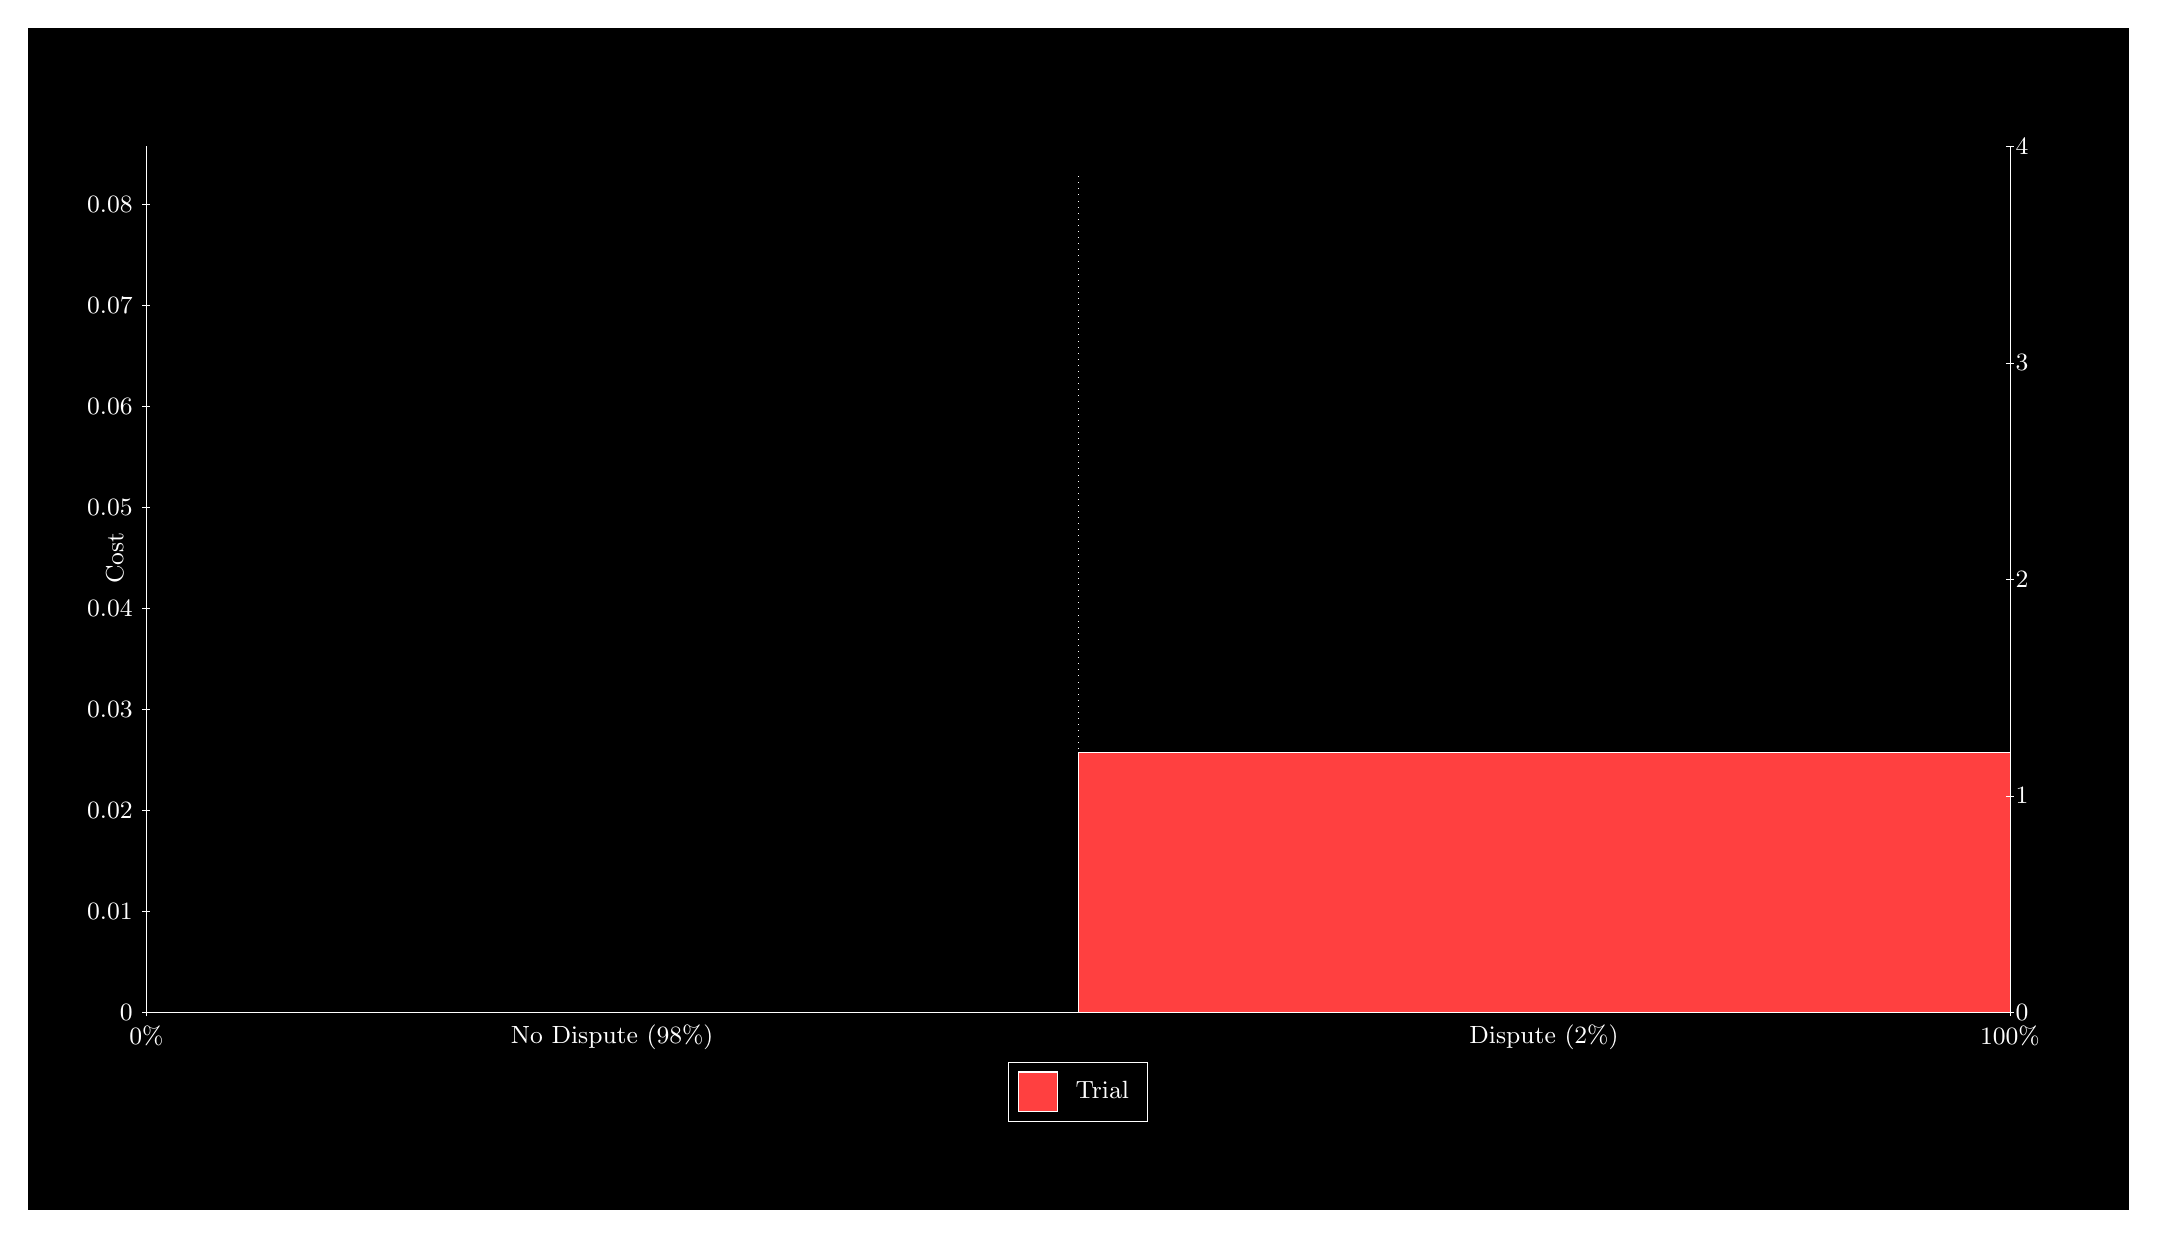
\begin{tikzpicture}
\draw[fill=black] (0,0) rectangle (26.667,15);
\draw[fill=red!75,draw=white,very thin] (13.333,2.5) rectangle (25.167,5.8);
\draw[white,very thin] (1.5,2.5) -- (1.5,13.5);
\node[font=\small,rotate=90,text=white, anchor=center] at (1.1, 8.2703) {Cost};
\draw[white,very thin] (1.45,2.5) -- (1.55,2.5);
\node[font=\small,text=white, anchor=east] at (1.45, 2.5) {0};
\draw[white,very thin] (1.45,3.7823) -- (1.55,3.7823);
\node[font=\small,text=white, anchor=east] at (1.45, 3.7823) {0.01};
\draw[white,very thin] (1.45,5.0646) -- (1.55,5.0646);
\node[font=\small,text=white, anchor=east] at (1.45, 5.0646) {0.02};
\draw[white,very thin] (1.45,6.3469) -- (1.55,6.3469);
\node[font=\small,text=white, anchor=east] at (1.45, 6.3469) {0.03};
\draw[white,very thin] (1.45,7.6292) -- (1.55,7.6292);
\node[font=\small,text=white, anchor=east] at (1.45, 7.6292) {0.04};
\draw[white,very thin] (1.45,8.9115) -- (1.55,8.9115);
\node[font=\small,text=white, anchor=east] at (1.45, 8.9115) {0.05};
\draw[white,very thin] (1.45,10.194) -- (1.55,10.194);
\node[font=\small,text=white, anchor=east] at (1.45, 10.194) {0.06};
\draw[white,very thin] (1.45,11.476) -- (1.55,11.476);
\node[font=\small,text=white, anchor=east] at (1.45, 11.476) {0.07};
\draw[white,very thin] (1.45,12.758) -- (1.55,12.758);
\node[font=\small,text=white, anchor=east] at (1.45, 12.758) {0.08};

\draw[white,dotted,very thin] (13.333,2.83) -- (13.333,13.17);
\draw[white,very thin] (25.167,2.5) -- (25.167,13.5);
\draw[white,very thin] (25.117,2.5) -- (25.217,2.5);
\node[font=\small,text=white, anchor=west] at (25.117, 2.5) {0};
\draw[white,very thin] (25.117,5.25) -- (25.217,5.25);
\node[font=\small,text=white, anchor=west] at (25.117, 5.25) {1};
\draw[white,very thin] (25.117,8) -- (25.217,8);
\node[font=\small,text=white, anchor=west] at (25.117, 8) {2};
\draw[white,very thin] (25.117,10.75) -- (25.217,10.75);
\node[font=\small,text=white, anchor=west] at (25.117, 10.75) {3};
\draw[white,very thin] (25.117,13.5) -- (25.217,13.5);
\node[font=\small,text=white, anchor=west] at (25.117, 13.5) {4};

\draw[white,very thin] (1.5,2.5) -- (25.167,2.5);
\draw[white,very thin] (1.5,2.45) -- (1.5,2.55);
\node[font=\small,text=white, anchor=north] at (1.5, 2.45) {0\%};
\draw[white,very thin] (25.167,2.45) -- (25.167,2.55);
\node[font=\small,text=white, anchor=north] at (25.167, 2.45) {100\%};

\node[font=\small,text=white,anchor=south] at (7.4167, 1.9) {No\ Dispute\ (98\%)};
\node[font=\small,text=white,anchor=south] at (19.25, 1.9) {Dispute\ (2\%)};
\draw (13.3333,2.5) node (B) {};
\begin{scope}[align=center]
\matrix[scale=0.5,draw=white,below=0.5cm of B,nodes={draw},column sep=0.1cm]{
\node[rectangle,draw,minimum width=0.5cm,minimum height=0.5cm,fill=red!75]{}; & \node[draw=none,font=\small,text=white]{Trial}; \\\\
};\end{scope}

\end{tikzpicture}
\end{document}